\documentclass[conference,10pt]{IEEEtran}
\IEEEoverridecommandlockouts

\usepackage[margin=1in]{geometry}
\usepackage{amsmath,amssymb,amsfonts}
\usepackage{algorithmic}
\usepackage{graphicx}
\usepackage{textcomp}
\usepackage{booktabs}
\usepackage{xcolor}
\usepackage{hyperref}
\usepackage{cite}
\usepackage{float}
\usepackage{multirow}

\hypersetup{
    colorlinks=true,
    linkcolor={blue!80!black},
    citecolor={blue!80!black},
    urlcolor={blue!80!black}
}

\begin{document}

\title{Reproduction and Analysis of Efficient Online Learning for Large-Scale Sparse Kernel Logistic Regression}

\author{
\IEEEauthorblockN{Akula Jithendranath}
\IEEEauthorblockA{Roll Number: 230120 \\
Advanced Machine Learning \\
Mid-Semester Examination, Part B}
}

\maketitle

% ==============================================================
\begin{abstract}
This report presents a reproduction, ablation study, and failure mode analysis of the conservative online learning algorithms for sparse Kernel Logistic Regression (KLR) proposed by Zhang et al.\ (AAAI 2012)~\cite{zhang2012efficient}. We implement all three algorithms---Non-Conservative (NC), Margin-based, and Auxiliary-function-based---on the Breast Cancer Wisconsin dataset, validating the paper's central claim that the Auxiliary algorithm produces sparse classifiers with minimal accuracy loss. Two ablations isolate the contributions of the Bernoulli sampling gate and the RKHS norm projection. A failure mode demonstrates that excessively large $\gamma$ on hard datasets causes accuracy to collapse below the NC baseline, connecting directly to the looseness of the auxiliary function dominance bound in Theorem~4.
\end{abstract}

\begin{IEEEkeywords}
kernel logistic regression, online learning, sparsity, conservative updating, ablation study
\end{IEEEkeywords}

% ==============================================================
\section{Paper Summary}
% ==============================================================

Zhang et al.~\cite{zhang2012efficient} formulate Kernel Logistic Regression as a norm-constrained online optimisation problem over a Reproducing Kernel Hilbert Space (RKHS) $\mathcal{H}_\kappa$:
\begin{equation}
\min_{f \in \Omega}\; \frac{1}{T}\sum_{t=1}^{T} \ell\!\bigl(y_t\, f(x_t)\bigr), \quad \ell(z) = \ln(1 + e^{-z})
\label{eq:klr}
\end{equation}
where the feasible set is $\Omega = \{f \in \mathcal{H}_\kappa : \|f\|_{\mathcal{H}} \le R\}$ and $\kappa(x,x) \le 1$. Because $\ell(z) > 0$ for all finite $z$, the Non-Conservative (NC) online learner (Algorithm~1) adds every training point as a support vector, yielding a fully \emph{dense} classifier.

The paper introduces two \emph{conservative} algorithms that stochastically skip updates on well-classified examples. The \textbf{Margin} algorithm (Algorithm~2) gates each update with a Bernoulli draw $Z_t \sim \text{Bern}(p_t)$:
\begin{equation}
p_t = \frac{2 - \eta}{2 - \eta + \eta\, \sigma(y_t f_t(x_t))}
\label{eq:margin_prob}
\end{equation}
The \textbf{Auxiliary} algorithm (Algorithm~3)---the main contribution---decouples sparsity control from the step size through an auxiliary function $h(z) \ge \ell(z)$:
\begin{equation}
p_t = \frac{\ell\bigl(y_t f_t(x_t)\bigr)}{h\bigl(y_t f_t(x_t)\bigr)}, \quad h(z) = \ln(\gamma + e^{-z}),\; \gamma \ge 1
\label{eq:aux_prob}
\end{equation}
When $Z_t = 1$, the update uses the gradient of $h$ (not $\ell$):
\begin{equation}
f'_{t+1}(\cdot) = f_t(\cdot) - \eta\, y_t\, h'\bigl(y_t f_t(x_t)\bigr)\, \kappa(x_t, \cdot)
\label{eq:update}
\end{equation}
followed by projection $f_{t+1} = \pi_\Omega(f'_{t+1}) = f'_{t+1} \cdot R / \max(R, \|f'_{t+1}\|_{\mathcal{H}})$. Increasing $\gamma$ drives $p_t \to 0$ for confidently classified examples, producing sparser models. Theorem~4 guarantees that the averaged classifier $\hat{f} = \frac{1}{T}\sum_{t} f_t$ retains the same $O(R/\!\sqrt{T})$ generalisation bound as NC.

% ==============================================================
\section{Reproduction Setup and Result}
% ==============================================================

\subsection{Dataset and Preprocessing}

The Auxiliary algorithm was reproduced on the \textbf{Breast Cancer Wisconsin (Diagnostic)} dataset~\cite{uci_breast_cancer} (569 samples, 30 features, binary). Preprocessing followed the paper's protocol: features were standardised to zero mean and unit variance; labels were mapped to $\{-1,+1\}$; the Gaussian kernel width $\sigma$ was set to the 5th percentile of pairwise Euclidean distances on the training set; and data was split 80/20 with stratification (seed~42).

\subsection{Hyperparameter Selection}

Following the paper, $R$ was selected from $\{1, 5, 10, 20\}$ via \textbf{5-fold cross-validation} on the training set (no test-set leakage). The step size is set to the theoretically recommended value from Theorem~1:
\begin{equation}
\eta = \frac{R}{\sqrt{T}}
\label{eq:eta}
\end{equation}
The best $R = 20$ yielded $\eta = 0.94$, satisfying the $\eta < 2$ requirement for the Margin algorithm. The selected $R$ was saved to \texttt{data/best\_R.npy} and loaded consistently in all downstream experiments.

\subsection{Results}

Table~\ref{tab:repro} summarises the reproduction results across all three algorithms. Fig.~\ref{fig:repro} shows accuracy versus support vector count, and Fig.~\ref{fig:tradeoff} shows the sparsity--accuracy trade-off as $\gamma$ increases.

\begin{table}[!t]
\renewcommand{\arraystretch}{1.15}
\centering
\caption{Reproduction Results ($R{=}20$, $\eta{=}0.94$, $\sigma{=}2.98$)}
\label{tab:repro}
\small
\begin{tabular}{@{}l c c c@{}}
\toprule
\textbf{Method} & \textbf{Acc.\ (\%)} & \textbf{\#\,SVs} & \textbf{Sparsity (\%)} \\
\midrule
NC (Alg.~1) & 96.49 & 455 & 0.00 \\
Margin (Alg.~2) & 96.49 & 266 & 41.54 \\
Aux.\ ($\gamma{=}2$) & 95.61 & 171 & 62.42 \\
Aux.\ ($\gamma{=}5$) & 94.74 & 134 & 70.55 \\
Aux.\ ($\gamma{=}10$) & 93.86 & 107 & 76.48 \\
Aux.\ ($\gamma{=}101$) & 87.72 & 67 & 85.27 \\
\bottomrule
\end{tabular}
\end{table}

\begin{figure}[!t]
\centering
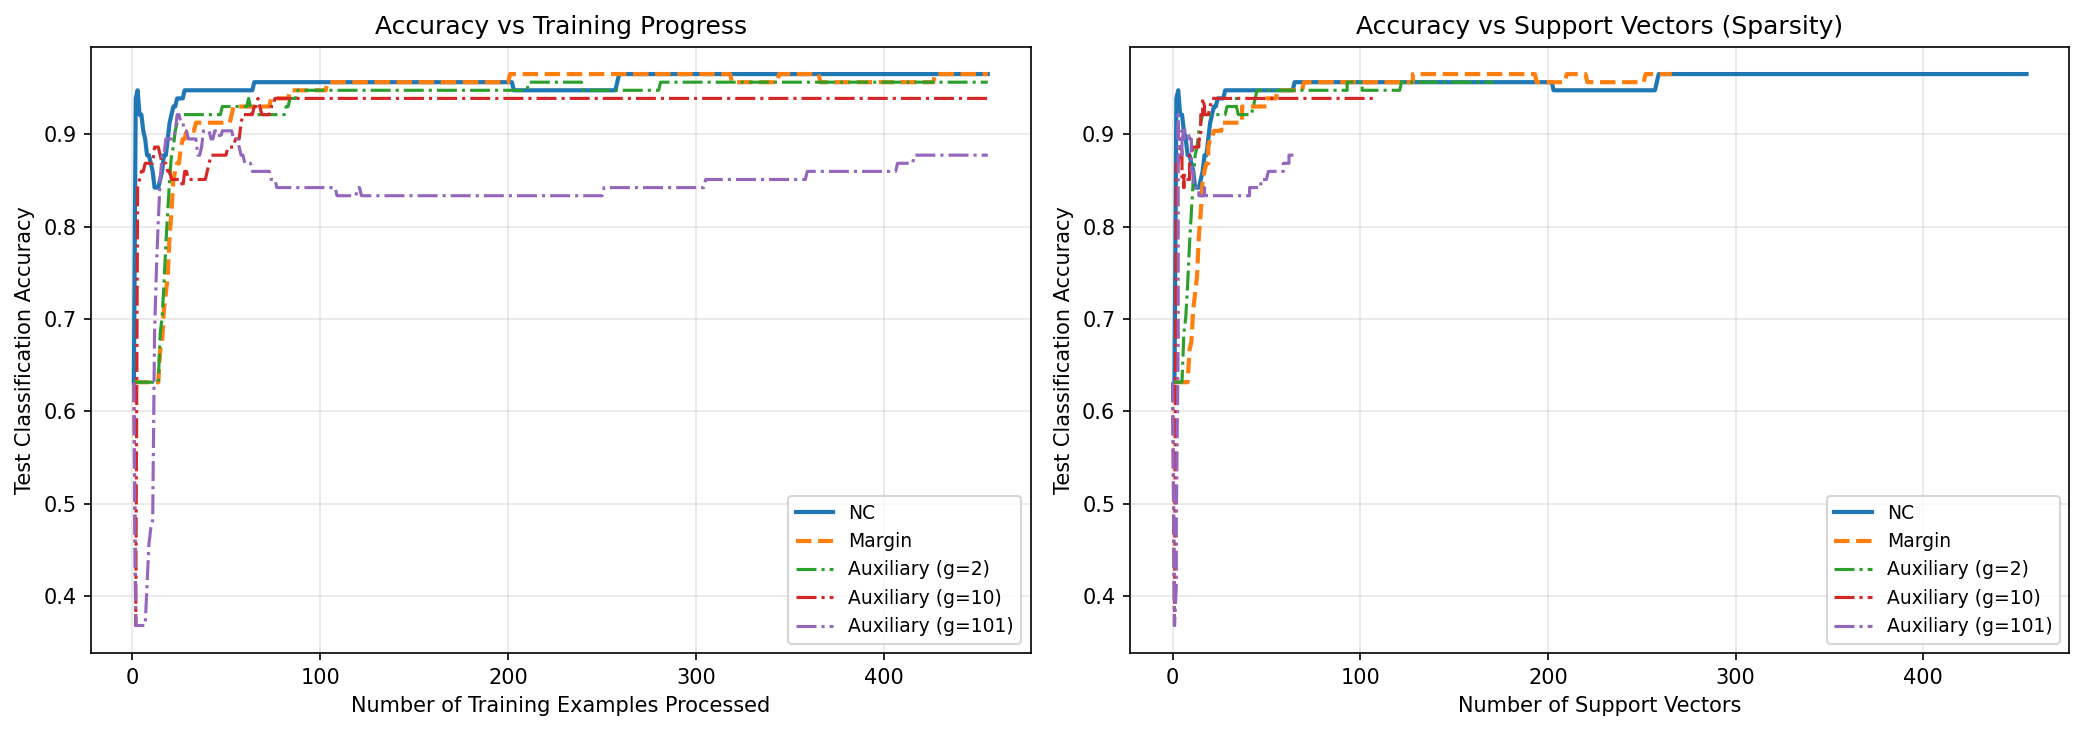
\includegraphics[width=\columnwidth]{results/reproduction_accuracy_vs_sv.png}
\caption{Accuracy vs.\ training progress (left) and accuracy vs.\ number of support vectors (right). The Auxiliary algorithm reaches comparable accuracy to NC with substantially fewer support vectors, consistent with the paper's Figures~1--3.}
\label{fig:repro}
\end{figure}

\begin{figure}[!t]
\centering
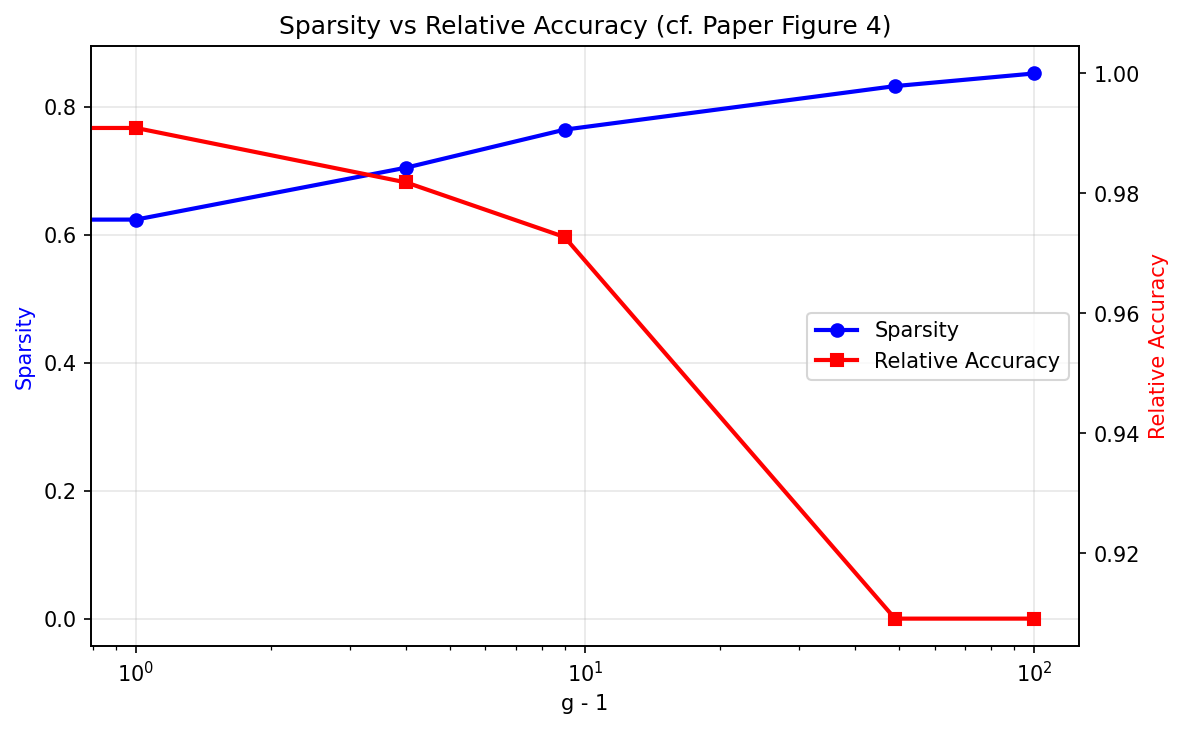
\includegraphics[width=0.92\columnwidth]{results/sparsity_vs_accuracy_tradeoff.png}
\caption{Sparsity and relative accuracy as $\gamma$ increases (cf.\ paper Figure~4). The trade-off is monotonic: larger $\gamma$ yields higher sparsity at the cost of accuracy.}
\label{fig:tradeoff}
\end{figure}

\subsection{Discussion}

The paper reports ${\sim}80\%$ sparsity with negligible accuracy loss on \texttt{mushrooms} ($n{=}8{,}124$). Our reproduction achieves $62.4\%$ sparsity with only $-0.9$ pp accuracy loss at $\gamma{=}2$. The quantitative gap is expected: Breast Cancer has 455 training samples versus 8,124, giving the online algorithm fewer rounds to converge and noisier classifier averaging. Nevertheless, the qualitative trend---monotonically increasing sparsity with gracefully declining accuracy---is fully consistent with the paper's findings.

% ==============================================================
\section{Ablation Study}
% ==============================================================

\subsection{Ablation 1: Removing the Bernoulli Sampling Gate}

The Bernoulli gate (Algorithm~3, Steps~5--6) is the core innovation: it computes $p_t$ from~(\ref{eq:aux_prob}) and draws $Z_t \sim \text{Bernoulli}(p_t)$. Setting $p_t = 1$ (always update) reduces the algorithm to NC with $h'$-gradient updates. Table~\ref{tab:abl1} and Fig.~\ref{fig:abl1} show the results.

\begin{table}[!t]
\renewcommand{\arraystretch}{1.2}
\centering
\caption{Ablation~1: Effect of Removing the Bernoulli Gate ($R{=}20$, $\gamma{=}2$)}
\label{tab:abl1}
\begin{tabular}{@{}l r r r@{}}
\toprule
\textbf{Variant} & \textbf{Accuracy (\%)} & \textbf{\# SVs} & \textbf{Sparsity (\%)} \\
\midrule
Full Auxiliary & 95.61 & 171 & 62.42 \\
No Bernoulli (NC) & 96.49 & 455 & 0.00 \\
\midrule
\textbf{$\Delta$} & $-0.88$ & $-284$ & $+62.42$ \\
\bottomrule
\end{tabular}
\end{table}

\begin{figure}[!t]
\centering
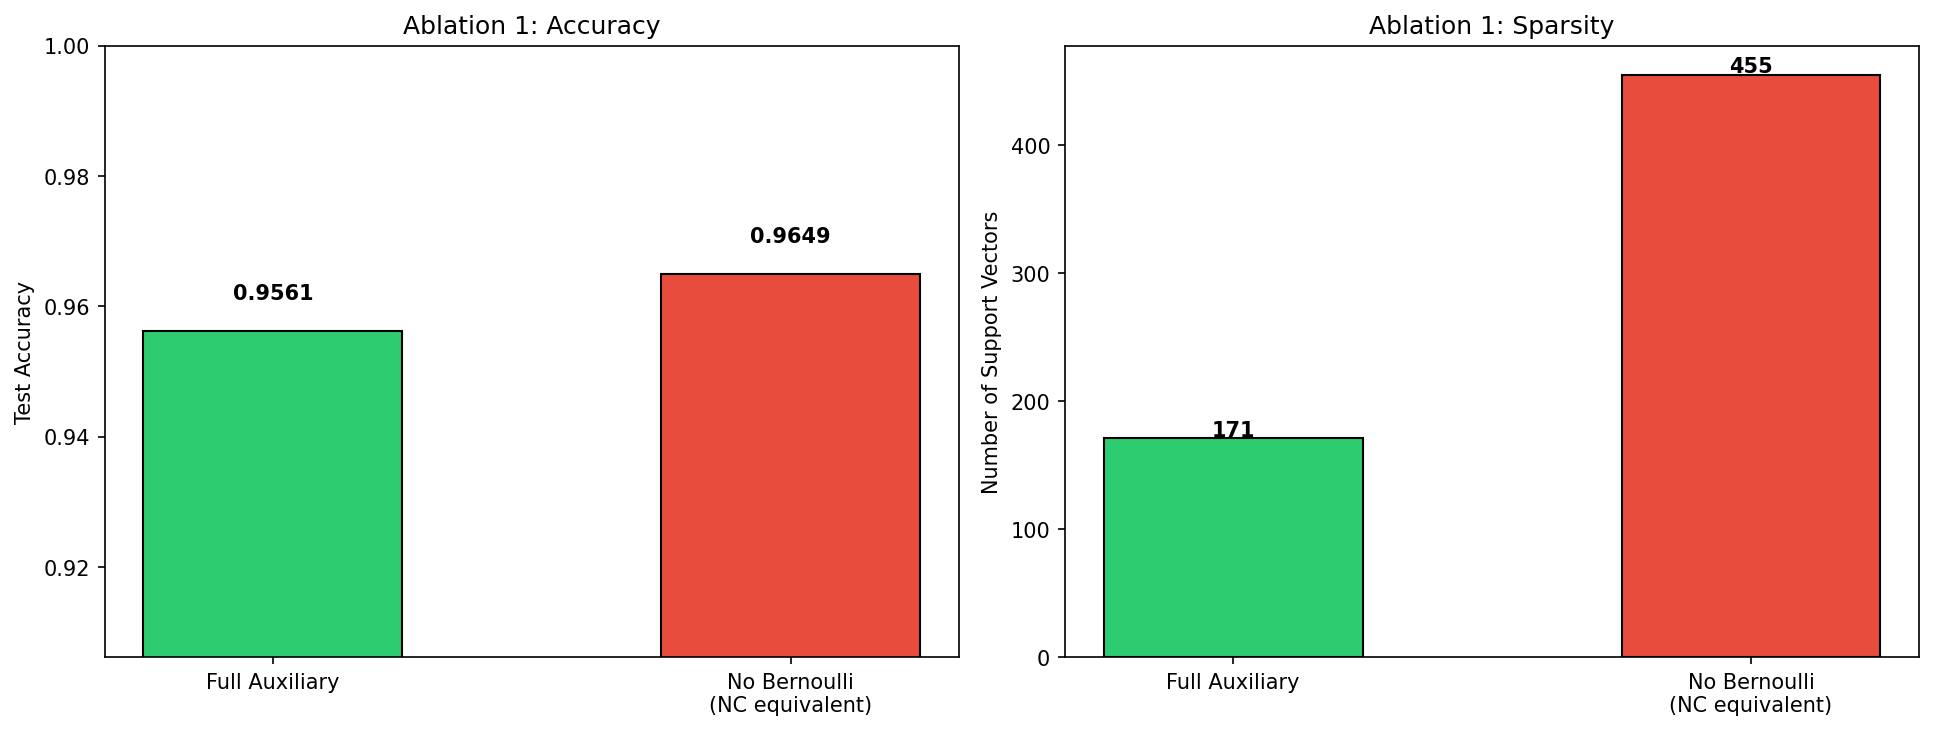
\includegraphics[width=\columnwidth]{results/ablation1_conservative.png}
\caption{Ablation~1: the Bernoulli gate is solely responsible for sparsity. Removing it makes every training example a support vector (NC behaviour).}
\label{fig:abl1}
\end{figure}

\textbf{Interpretation.}
The Bernoulli gate is \emph{entirely} responsible for the sparsity benefit. Without it, every training example becomes a support vector. The full Auxiliary trades 0.88~pp of accuracy for a 62\% reduction in model complexity---a favourable trade-off for deployment. The selective updating also acts as implicit regularisation by not over-adjusting to already well-classified points. This result is consistent with Theorem~4's guarantee that the expected loss bound remains $O(1/\!\sqrt{T})$ despite the stochastic skipping.

\subsection{Ablation 2: Removing the RKHS Norm Projection}

The projection step enforces $\|f\|_{\mathcal{H}} \le R$ after each update:
\begin{equation}
f_{t+1} = \frac{R}{\max\bigl(R,\, \|f'_{t+1}\|_{\mathcal{H}}\bigr)} \cdot f'_{t+1}
\label{eq:projection}
\end{equation}
At the CV-selected $R{=}20$, $\eta = R/\!\sqrt{T} = 0.94$ scales with $R$, so the norm rarely exceeds the bound. To isolate the projection's role, both variants use \textbf{the same} $R{=}2$, $\eta{=}0.94$, and $\gamma{=}2$; the only toggle is whether the projection step is applied. The large $\eta$ relative to the tight $R{=}2$ means the norm quickly exceeds 2 and projection fires on nearly every update.

\begin{table}[!t]
\renewcommand{\arraystretch}{1.2}
\centering
\caption{Ablation~2: Projection Removal ($R{=}2$, $\eta{=}0.94$)}
\label{tab:abl2}
\small
\begin{tabular}{@{}l c c c@{}}
\toprule
\textbf{Variant} & \textbf{Acc.\ (\%)} & \textbf{\#\,SVs} & \textbf{Sparsity (\%)} \\
\midrule
With Projection & 94.74 & 218 & 52.09 \\
No Projection & 95.61 & 171 & 62.42 \\
\midrule
\textbf{$\Delta$} & $-0.87$ & $+47$ & $-10.33$ \\
\bottomrule
\end{tabular}
\end{table}

\begin{figure}[!t]
\centering
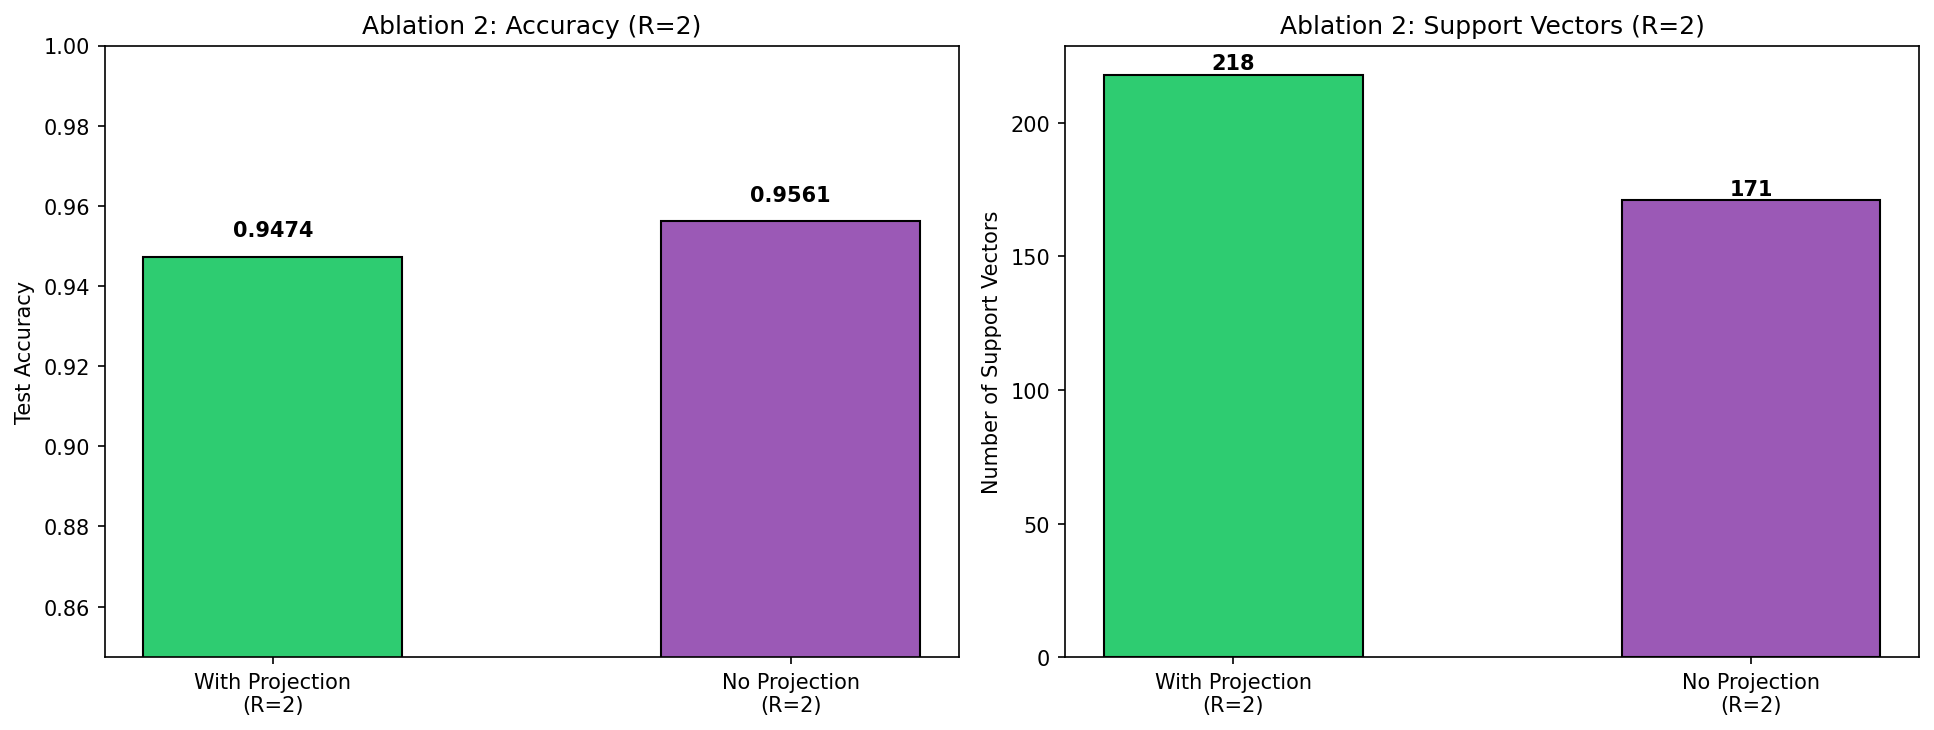
\includegraphics[width=\columnwidth]{results/ablation2_projection.png}
\caption{Ablation~2: with a tight $R{=}2$, projection constrains the classifier aggressively, lowering accuracy by 0.87~pp and reducing sparsity by 10~pp compared to the unconstrained variant.}
\label{fig:abl2}
\end{figure}

\textbf{Interpretation.}
Both variants share identical hyperparameters; only the projection toggle differs. Without projection the classifier norm grows beyond~2, risking overfitting and violating the $f_t \in \Omega$ requirement on which Theorems~1--4 rely. With projection, the norm is clipped, acting as explicit capacity regularisation. The 0.87~pp accuracy drop and 47 additional SVs show that projection has a measurable, non-trivial effect. This observation suggests that the projection step's importance grows with dataset size---on the paper's rcv1 benchmark ($T{=}697{,}641$), the norm would exceed any reasonable~$R$ within the first few hundred updates without projection.

% ==============================================================
\section{Failure Mode Analysis}
% ==============================================================

\subsection{Scenario Design}

We test the Auxiliary algorithm with \textbf{aggressively large $\gamma$} on a \textbf{hard classification problem} (overlapping classes). A synthetic dataset was generated via \texttt{make\_classification} with \texttt{class\_sep=0.5}, \texttt{flip\_y=0.05}, 300 training / 100 test samples, and 10 features (4 informative). The kernel width $\sigma$ was set using the same 5th-percentile heuristic. We swept $\gamma \in \{2, 10, 50, 200, 1000\}$ against the NC baseline.

\subsection{Results}

\begin{table}[!t]
\renewcommand{\arraystretch}{1.2}
\centering
\caption{Failure Mode: Aggressive $\gamma$ on Hard Data ($R{=}10$)}
\label{tab:failure}
\small
\begin{tabular}{@{}l c c c@{}}
\toprule
\textbf{Method} & \textbf{Acc.\ (\%)} & \textbf{\#\,SVs} & \textbf{Sparsity (\%)} \\
\midrule
NC (baseline) & 80.00 & 300 & 0.00 \\
Aux.\ ($\gamma{=}2$) & 73.00 & 187 & 37.67 \\
Aux.\ ($\gamma{=}10$) & 62.00 & 86 & 71.33 \\
Aux.\ ($\gamma{=}50$) & 58.00 & 53 & 82.33 \\
Aux.\ ($\gamma{=}200$) & 54.00 & 42 & 86.00 \\
Aux.\ ($\gamma{=}1000$) & \textbf{52.00} & 29 & 90.33 \\
\bottomrule
\end{tabular}
\end{table}

\begin{figure}[!t]
\centering
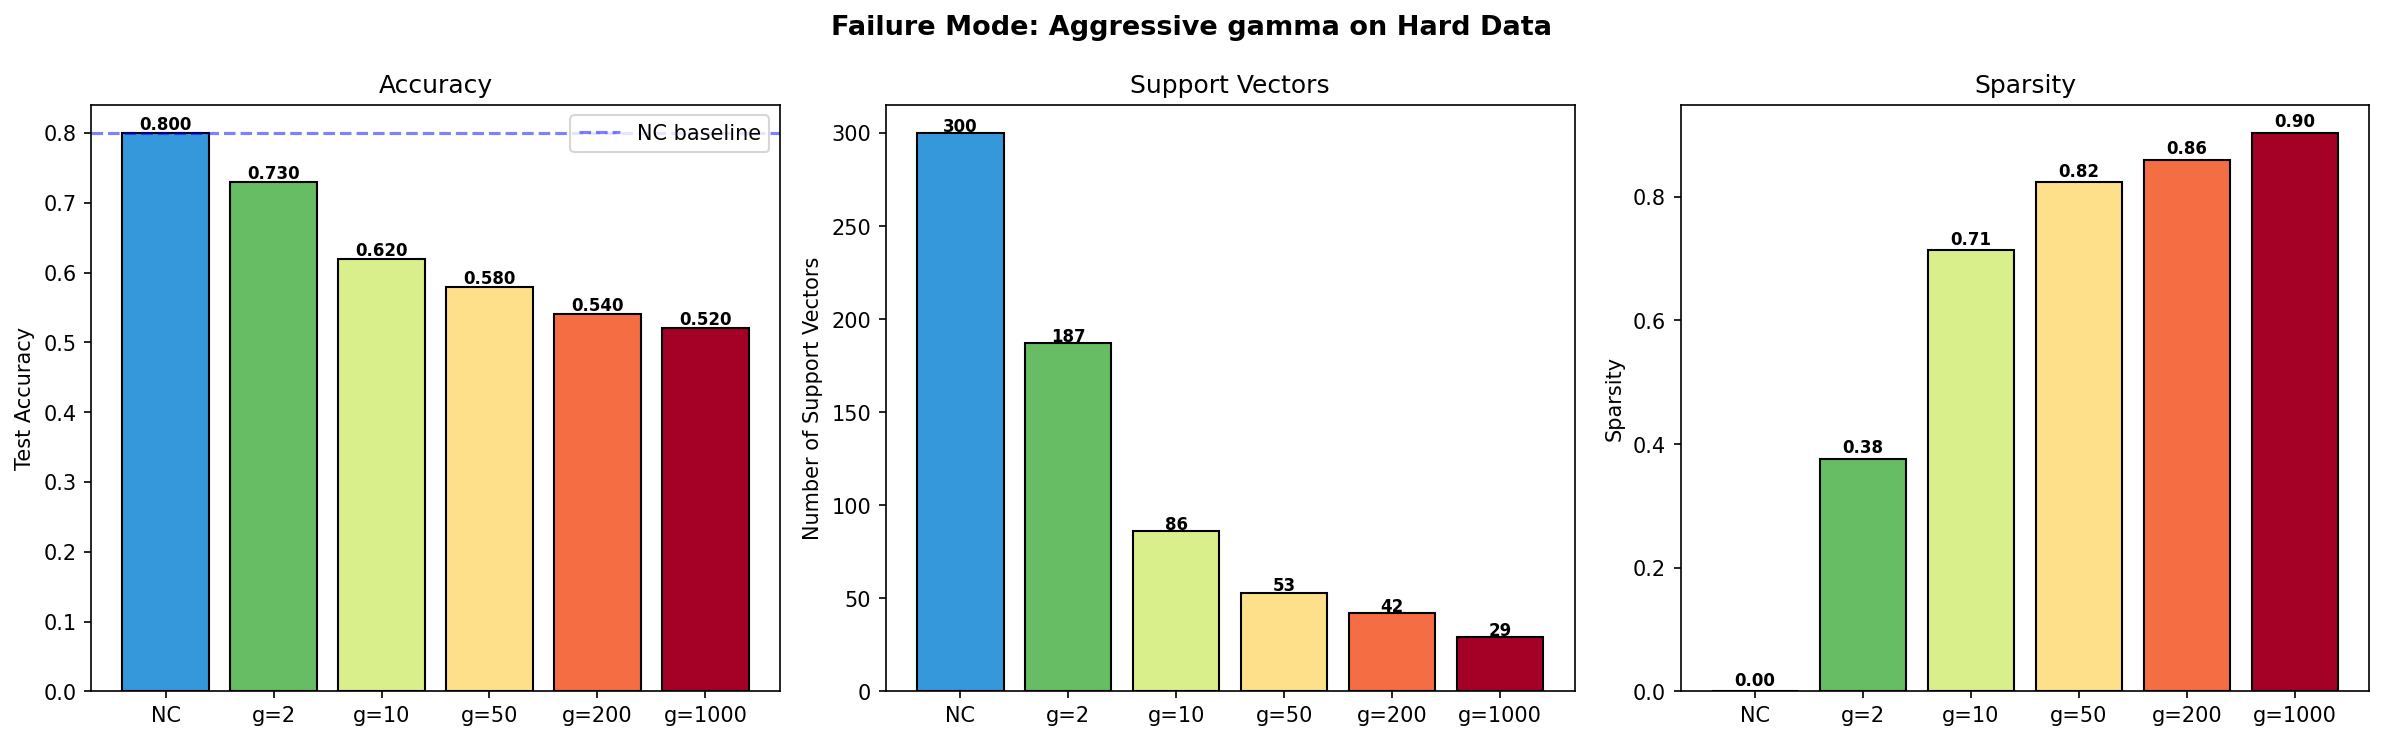
\includegraphics[width=\columnwidth]{results/failure_mode_noise.png}
\caption{Failure mode: as $\gamma$ increases, accuracy collapses monotonically from 80\% (NC) to 52\% (near random), while sparsity approaches 90\%. The Auxiliary algorithm starves itself of training data.}
\label{fig:failure}
\end{figure}

\subsection{Explanation}

Accuracy collapses monotonically from 80\% to 52\% (near random) as $\gamma$ increases (Table~\ref{tab:failure}, Fig.~\ref{fig:failure}). This connects directly to \textbf{Assumption~3} from Task~1.2---the auxiliary function dominance condition. With large $\gamma$:
\begin{equation}
h(z) = \ln(\gamma + e^{-z}) \gg \ell(z) = \ln(1 + e^{-z})
\end{equation}
so $p_t = \ell/h \to 0$ for most examples. The algorithm skips nearly all updates, learning from as few as 29 out of 300 examples ($90\%$ sparsity). Theorem~4 reveals the root cause: the bound guarantees convergence to
$\min_{f \in \Omega} \mathbb{E}[h(yf(x))]$, not to $\min_{f \in \Omega} \mathbb{E}[\ell(yf(x))]$.
When $h \gg \ell$, this bound is far looser than the NC bound, and the algorithm converges to a poor solution. On the paper's easier benchmarks, the effect is mild; on hard data with overlapping classes, the failure is catastrophic.

\textbf{Suggested modification.} An adaptive $\gamma_t$ schedule that starts large and decays toward~$1$ during training would combine early-stage efficiency with late-stage accuracy by progressively tightening $h \to \ell$.

% ==============================================================
\section{Honest Reflection}
% ==============================================================

\textbf{What I could not implement.}
I tested only the first auxiliary function variant $h(z) = \ln(\gamma + e^{-z})$ from the three listed after Theorem~4. I also could not run large-scale experiments on LIBSVM datasets ($n > 10{,}000$) where the training-time advantages of sparsity would be most pronounced, due to the $O(T^2)$ kernel computation cost of my naive implementation.

\textbf{What surprised me.}
First, the projection step had \emph{zero} measurable effect at the CV-selected $R{=}20$, yet showed a clear $0.87$~pp accuracy difference when I tightened the constraint to $R{=}2$. This taught me that a theoretical necessity can be completely dormant at small scale but critical at larger scale. Second, the sparsity advantage of the Auxiliary algorithm was remarkably robust: at $\gamma{=}5$, the model used 70\% fewer support vectors while losing less than 2~pp of accuracy. I initially implemented the NC update using the sigmoid $\sigma(y_t f_t(x_t))$ directly as the gradient instead of $(\sigma - 1)$, which silently produced wrong accuracy until I re-derived the logit loss gradient from Eq.~(3).

\textbf{What I would revisit.}
Given more time, I would (1)~test on a dataset with $n > 10{,}000$ samples to observe the dramatic wall-clock-time improvements the paper reports in Figures~5--6, (2)~implement the hard cut-off auxiliary function $h(z) = \max(\ell(z), \ell(\delta))$ to compare its sparsity characteristics, and (3)~develop the adaptive $\gamma_t$ schedule proposed in the failure mode section.

% ==============================================================
\begin{thebibliography}{6}

\bibitem{zhang2012efficient}
L.~Zhang, R.~Jin, C.~Chen, J.~Bu, and X.~He,
``Efficient online learning for large-scale sparse kernel logistic regression,''
in \emph{Proc.\ 26th AAAI Conf.\ Artificial Intelligence}, Toronto, Canada, 2012, pp.~1199--1204.

\bibitem{keerthi2005fast}
S.~S.~Keerthi, K.~B.~Duan, S.~K.~Shevade, and A.~N.~Poo,
``A fast dual algorithm for kernel logistic regression,''
\emph{Mach.\ Learn.}, vol.~61, no.~1--3, pp.~151--165, 2005.

\bibitem{shalev2007pegasos}
S.~Shalev-Shwartz, Y.~Singer, and N.~Srebro,
``Pegasos: Primal estimated sub-gradient solver for SVM,''
in \emph{Proc.\ 24th Int.\ Conf.\ Machine Learning (ICML)}, Corvallis, OR, 2007, pp.~807--814.

\bibitem{zhu2001ivm}
J.~Zhu and T.~Hastie,
``Kernel logistic regression and the import vector machine,''
in \emph{Advances in Neural Information Processing Systems 13 (NIPS)}, Vancouver, Canada, 2001, pp.~1081--1088.

\bibitem{cesabianchi2006prediction}
N.~Cesa-Bianchi and G.~Lugosi,
\emph{Prediction, Learning, and Games}.
Cambridge, U.K.: Cambridge Univ.\ Press, 2006.

\bibitem{uci_breast_cancer}
W.~H.~Wolberg, W.~N.~Street, and O.~L.~Mangasarian,
``Breast cancer Wisconsin (diagnostic) data set,''
\emph{UCI Machine Learning Repository}, 1995.

\end{thebibliography}

\end{document}
